\documentclass{scrartcl}
\usepackage[utf8]{inputenc}
\usepackage{graphicx}
\usepackage{float}
\usepackage[T1]{fontenc}
\usepackage{listings}
\usepackage{babel}

\title{Rice cooker model}
\author{Peter Bence\\X89O8X}
\date{October 2022}

\begin{document}

\maketitle
\newpage

\tableofcontents
\newpage

\section{Description}
This is a model of a multifunctional rice cooker. This rice cooker have a digital display, 8 special cooking functions and a keep warm function. It will cook all kinds of rice perfectly and will also take care of the cooking of other dishes. With the cooker comes a stirring spoon, a ladle, a measuring cup and a basket for steaming vegetables. With this documentation of the device, I hope the reader can understand the functions and the use cases of this machine.

\section{Use cases}
\begin{table}[H] \centering
    \caption{Use cases}\label{tab:usecasetable}
    \begin{tabular}{@{}ll@{}} \hline
        \emph{Case} & \emph{Description}\\
        1. Cook quick rice & Cook jasmin or other quick rice types in 10-15 minutes.\\
        2. Cook white rice & Cook normal rice in 45-60 minuntes.\\
        3. Cook brown rice & Cook brown rice in 45 minutes.\\
        4. Cook pouridge & Cook oatmeal in 10 minutes.\\
        5. Cook soup & Cook soup.\\
        6. Steam vegetables & Steam vegetables.\\
        7. Cook rice and vegetables & Cook rice and cook vegetables at the same time.\\
        8. Manual program & Set timer manually, how long the cooker should cook.
    \end{tabular}
\end{table}
\begin{figure}[H]\centering
    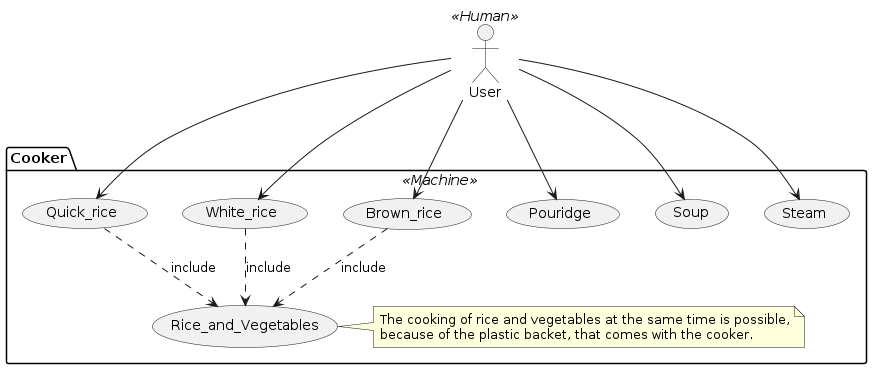
\includegraphics[width=1.1\columnwidth]{UseCase.png}
    \caption{Use Cases}\label{fig:1}
\end{figure}

\newpage

\section{Requirements}
\begin{table}[H] \centering
    \caption{Requirements}\label{tab:requirementstable}
    \begin{tabular}{@{}ll@{}} \hline
        \emph{Case} & \emph{Description}\\
        Cook quick rice & Be able to cook jasmin or other quick rice types quicker.\\
        Cook white rice & Have normal rice cooking program. \\
        Cook brown rice & Have separate brown rice cooking program.\\
        Cook pouridge & Have oatmeal cooking program that cooks oatmeal.\\
        Cook soup & Have a soup cooking program that can cook soup with meat.\\
        Steam vegetables & Have a steaming program that can make steamed vegetables.\\
        Cook rice and vegetables & Be able to cook rice and cook vegetables at the same time.\\
        Steam & Have a plastic basket for steaming vegetables.\\
        Manual & Can set manually the cooking time.\\ 
        Non-stick surface & The cooking bowl must have a non stick surface.\\
        Plastic tools & Have plastic tools that comes with the rice cooker,\\ & ex.: stirring spoon, measuring cup, etc.
    \end{tabular}
\end{table}

\section{Machine Structure}
\subsubsection{Components}
\begin{figure}[H]\centering
    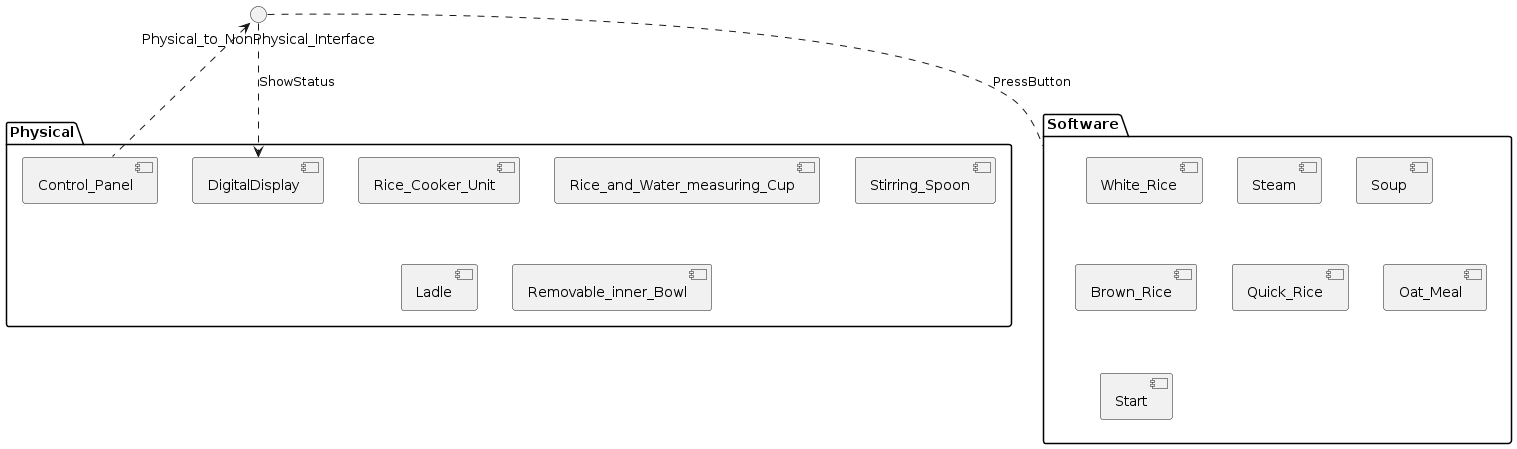
\includegraphics[width=1.2\columnwidth]{Component.png}
    \caption{component}\label{fig:2}
\end{figure}

\section{Behaviour}
\subsubsection{StateMachine}
\begin{figure}[H]\centering
    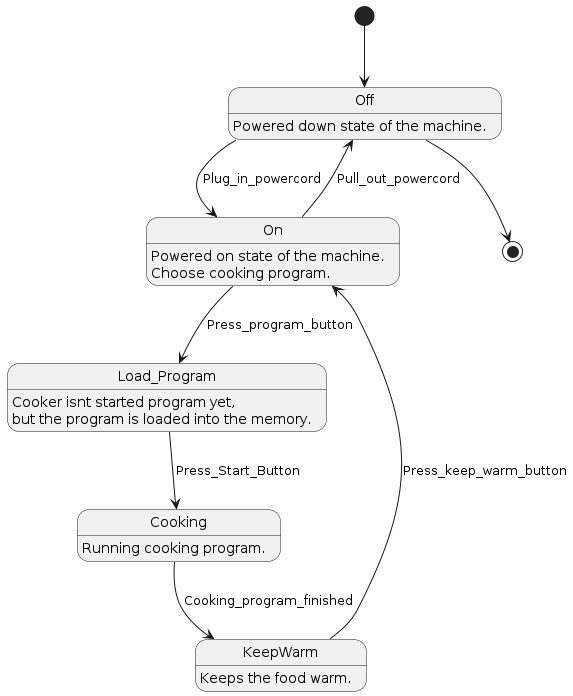
\includegraphics[width=1.1\columnwidth]{StateMachine.png}
    \caption{statemachine}\label{fig:3}
\end{figure}

\subsubsection{Sequences}
\begin{figure}[H]\centering
    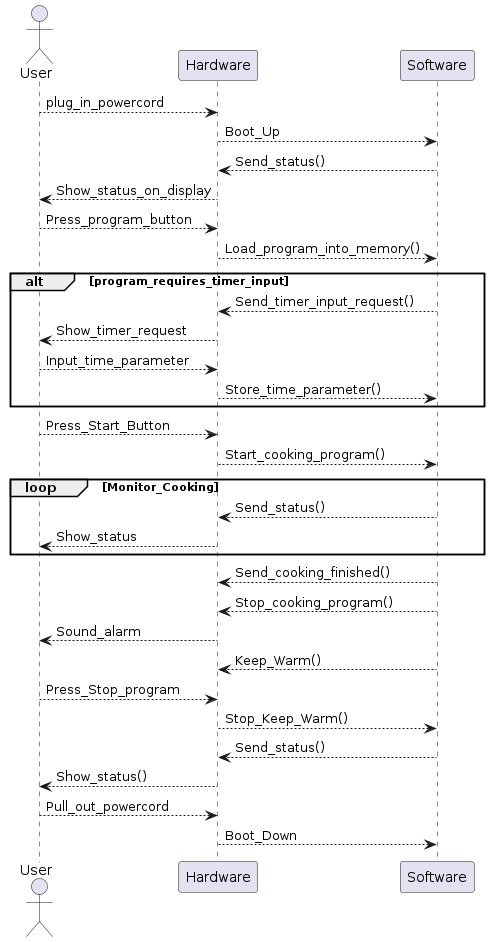
\includegraphics[width=0.65\columnwidth]{Sequence.png}
    \caption{sequence}\label{fig:4}
\end{figure}

\end{document}